\documentclass[sigconf]{acmart}

% \renewcommand\footnotetextcopyrightpermission[1]{} % removes footnote with conference information in first column
\pagestyle{fancy} % removes running headers

\setlength{\parskip}{0pt}
\setlength{\parsep}{0pt}
\setlength{\headsep}{0pt}
\setlength{\topskip}{0pt}
\setlength{\topmargin}{0pt}
\setlength{\topsep}{0pt}
\setlength{\partopsep}{0pt}
%\linespread{0.95}
\usepackage{mdwlist}

\usepackage{amsmath}
\fancyhead{}
\settopmatter{printacmref=false, printfolios=false}
% Copyright
\setcopyright{none}
% \setcopyright{acmcopyright}
% \setcopyright{acmlicensed}
% \setcopyright{rightsretained}
% \setcopyright{usgov}
% \setcopyright{usgovmixed}
% \setcopyright{cagov}
% \setcopyright{cagovmixed}

\settopmatter{printacmref=false} % Removes citation information below abstract
\begin{document}
\title{Minimum Edit Distance Performance for Auto-spell Correction}
\titlenote{\href{https://github.com/duongy18418/NLP-Assignments}{https://github.com/duongy18418/NLP-Assignments}}

\author{Miaomiao Zhang}
% \authornotemark[1]
\affiliation{
 \institution{University of Windsor}
%   \city{Fredericton} 
%   \state{NB} 
%   \country{Canada} 
}\email{zhang3s2@uwindsor.ca}

\author{Kitty Duong}
% \authornotemark[1]
\affiliation{
 \institution{University of Windsor}
%   \city{Fredericton} 
%   \state{NB} 
%   \country{Canada} 
}\email{duongy@uwindsor.ca}

\maketitle

\section{Introduction}
Many tasks in Natural Language Processing are concerned with measuring how similar two strings are. The Minimum Edit Distance (MED) algorithm, also known as the Levenshtein distance or the edit distance, is a measure of the minimum number of editing operations needed to transform one string to another one. The Levenshtein Distance and the underlying ideas are widely used in areas like computer science, computer linguistics, and even bio-informatics, molecular biology, and DNA analysis. As for the dictionary in this experiment, we would use PyDictionary, which is a Dictionary Module for Python, using WordNet to get meanings, translations, synonyms, and Antonyms of words. Birkbeck would be the spelling error corpus, which includes the most common misspelled tokens and the correct spell in pairs.

\section{Motivation}
The Minimum Edit Distance (MED) algorithm is a versatile tool that is widely applied in various fields where measuring the similarity or dissimilarity between sequences is crucial. This algorithm is designed to quantify the cost of transforming one sequence into another making it valuable in solving a wide range of computational problems. In Natural Language Processing and spell-checking applications, the MED algorithm is used to suggest corrections for misspelled words. It helps identify the minimum number of edits needed to convert a misspelled word into a correctly spelled one.

\section{Problem Definition}
Given WordNet as the dictionary $\mathcal{D}$ and Birkbeck as the corpus of misspelled tokens $\mathcal{C}$, and a random token $t\in \mathcal{C}$, the goal is to calculate the average success at k (s@k), k={1, 5, 10}, for the minimum edit distance (MED) algorithm for all misspelled tokens in C.

\subsection{Example}
For instance, given "desing" from Birkbeck corpus, the top-5 most similar (least distant) tokens to 'desing' based on MED from WordNet are ['desi', 'design', 'designer', 'designate', 'despair']. Then, s@1 is 0 since the correct spell from Birkbeck is 'design' which is not happening at the first item. However, s@k is 1 when k is greater or equal to 2.

\section{Experiment}
\subsection{Datasets}
In this experiment, we used two datasets, the first dataset is the "Birkbeck" spelling error corpus. This contains a list of misspelled words along with their correct spellings. The second one is "Wordnet", which consists of a list of all English words against which we compare our misspelled words in this experiment.

\subsection{Results}
Based on the Minimum Edit Distance (MED) Algorithm, we divided this problem into two sub-problems, thus there are two parts of the final solution algorithm. In the first part, we intended to take the incorrect spellings and return the correct similar tokens from the WordNet dictionary.

\begin{figure}[h]
    \centering
    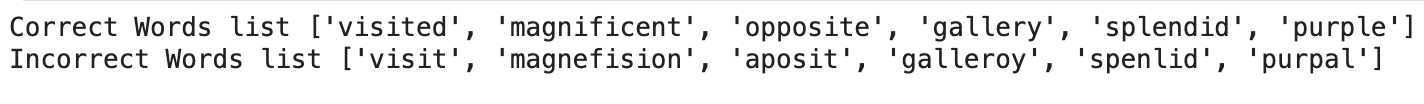
\includegraphics[width=1.1\linewidth]{correct_words.png}
    \caption{correct tokens output}
    \label{fig:enter-label}
\end{figure}

The second part aims to return a list of only k(k = 1, 5, 10) numbers of tokens. For instance, for the token "gallery", the output is:
\begin{enumerate}
    \item s@k for k = 1:  0.15789473684210525
    \item s@k for k = 5:  0.0
    \item s@k for k = 10:  0.0
\end{enumerate}

For the final output for the tokens from the Birkbeck Spelling corpus, we take k values from (1,5,10). The average probability of s@10 is the highest among the three types of values.

\begin{figure}[h]
    \centering
    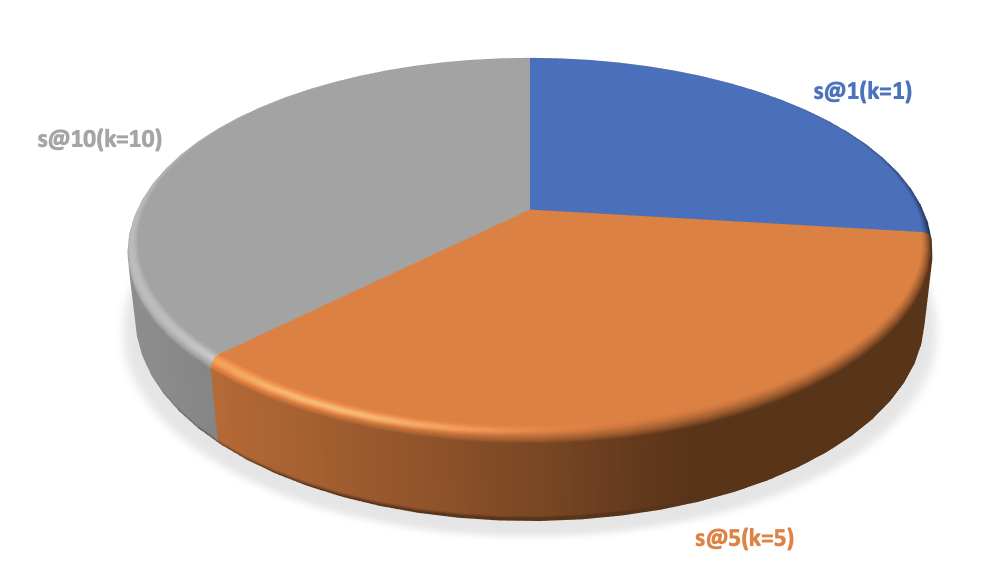
\includegraphics[width=0.7\linewidth]{final_res.png}
    \caption{average s@k output}
    \label{fig:enter-label}
\end{figure}

\section{Conclusion and Future Direction}
The Minimum Edit Distance (MED) algorithm is a dynamic programming algorithm commonly used in natural language processing for spell-checking and related fields. It could also be used in machine learning techniques, especially deep learning with further advancements in algorithm efficiency in the future.

\bibliographystyle{ACM-Reference-Format}
\bibliography{bibliography.bib} 
\textit{https://en.wikipedia.org/wiki/WordNet}\\
\textit{https://ota.bodleian.ox.ac.uk/repository/xmlui/handle/20.500.12024/0643}
\end{document}

